\section{Снижение взлома награды с помощью проверяемых композитных функций награды}
\subsection{Ключевые идеи}

Основная задача статьи~\cite{tarek2025rewardhackingmitigationusing} 
состоит в снижении взлома награды при обучении больших языковых моделей для 
решения медицинских задач множественного выбора в рамках схемы обучения с 
подкреплением с проверяемой наградой. Модель должна формировать рассуждение 
внутри тегов \verb|<think>...</think>| и выдавать финальный вариант ответа только
внутри \verb|<answer>...</answer>|. Однако при прямом применении такой схемы 
возникают два характерных вида нежелательного поведения: преждевременное 
раскрытие ответа в блоке рассуждения и структурные нарушения, включающие 
вывод рассуждений вне \verb|<think>| или чрезмерно длинный пролог перед 
этим тегом.

Для устранения подобных дефектов авторы вводят \emph{композитную функцию награды}, 
которая сочетает бинарную награду за правильный ответ с двумя специально 
сконструированными штрафами: за семантическое утекание ответа и за нарушение 
структуры вывода (например, чрезмерную длину текста перед \verb|<think>|). 
В совокупности эта функция награды направлена на то, чтобы модель не только 
получала высокую итоговую награду, но и формировала рассуждение и ответ строго 
в предписанном формате.

Композитная награда используется совместно с методом REINFORCE и сетью-базисом 
для стабилизации оценки преимущества. Общая структура метода представлена на 
Рисунке~\ref{fig:Comp_RM}.


\subsection{Математическое описание метода}

Пусть $g$ обозначает одну сгенерированную моделью последовательность 
(ответ) на заданный медицинский вопрос. В композитной функции награды 
учитываются три компоненты:

\begin{itemize}
    \item бинарная награда $R_{\text{binary}}(g)$ за корректность и формат ответа;
    \item штраф за преждевременное раскрытие ответа $P_{\text{answer}}(g)$;
    \item штраф за структурное нарушение $P_{\text{structural}}(g)$.
\end{itemize}

\begin{equation}
    R_{\text{total}}(g) = w_b R_{\text{binary}}(g) 
    - w_a P_{\text{answer}}(g) 
    - w_s P_{\text{structural}}(g),
\end{equation}
где $w_b, w_a, w_s > 0$~-- веса, задающие важность каждой компоненты.

\paragraph{Бинарная награда за корректность ответа.}

Пусть $a_g$~-- финальный вариант ответа, извлечённый из тега \verb|<answer>| 
в генерации $g$, а $a^*$~-- правильный вариант ответа из разметки. Тогда 
бинарная награда задаётся как
\begin{equation}
R_{\text{binary}}(g)
=
\begin{cases}
+1, & \text{если } a_g = a^* \text{ и формат корректен},\\
0,  & \text{если } a_g \neq a^* \text{ и формат корректен},\\
-1, & \text{если } a_g \neq a^* \text{ и формат некорректен}.
\end{cases}
\end{equation}

Таким образом, модель поощряется за правильный ответ в заданном формате и 
дополнительно наказывается, если при неправильном ответе формат также нарушен.

\paragraph{Штраф за преждевременное раскрытие ответа.}

Пусть $t_{\text{think}}$~-- текст внутри блока \verb|<think> ... </think>| 
в генерации $g$. Используется заранее обученная модель для эмбеддингов 
редложений (например, вариант «двойного» трансформера для предложений), 
которая сопоставляет каждому тексту вектор в евклидовом пространстве.

Заранее фиксируется набор из $m$ типичных фраз, прямо или косвенно 
объявляющих ответ (\emph{фразы утечки}), например:
\begin{itemize}
    \item «правильный ответ~--»,
    \item «ответ~-- вариант C»,
    \item «мы приходим к выводу, что ответ B» и т.\,п.
\end{itemize}

Обозначим этот набор через $L = \{l_1, \dots, l_m\}$, а функцию получения 
эмбеддингов через $E(\cdot)$. Тогда:
\begin{itemize}
    \item вычисляются эмбеддинги всех фраз утечки $E(l_i)$;
    \item вычисляется эмбеддинг блока рассуждения 
    $v_{\text{think}} = E(t_{\text{think}})$;
    \item рассчитывается максимальное косинусное сходство между 
    $v_{\text{think}}$ и любым $E(l_i)$:
\end{itemize}

\begin{equation}
    S_{\text{answer}}(g) 
    = \max_{i=1,\dots,m} \operatorname{Sim}\!\bigl( v_{\text{think}}, E(l_i) \bigr),
\end{equation}
где $\operatorname{Sim}(\cdot,\cdot)$~-- косинусное сходство.

Штраф определяется как
\begin{equation}
P_{\text{answer}}(g)
=
\begin{cases}
S_{\text{answer}}(g), & \text{если } S_{\text{answer}}(g) > \tau_{\text{answer}},\\
0, & \text{иначе},
\end{cases}
\end{equation}
где $\tau_{\text{answer}} \in (0,1)$~-- заданный порог. Чем сильнее 
рассуждение похоже на утекающую фразу, тем выше штраф.

\paragraph{Штраф за структурное нарушение.}

Пусть $T_{\text{preamble}}$~-- текст, сгенерированный до первого 
появления тега \verb|<think>|. Считается число слов $|T_{\text{preamble}}|$. 
Если оно превышает порог $\tau_{\text{preamble}}$, назначается фиксированный 
штраф $\lambda_s$:
\begin{equation}
    P_{\text{structural}}(g)
    =
    \begin{cases}
    \lambda_s, & \text{если } |T_{\text{preamble}}| > \tau_{\text{preamble}},\\
    0, & \text{иначе}.
    \end{cases}
\end{equation}

Это стимулирует модель не «уходить» в длинные введения с рассуждениями вне 
тега \verb|<think>|.

\paragraph{Обучение политики методом REINFORCE.}

Пусть $\pi_\theta(a \mid s)$~-- стохастическая политика модели: вероятность 
сгенерировать последовательность действий $a = (a_1, \dots, a_T)$ 
при условии входного состояния (промпта) $s$. Обозначим суммарную награду 
за генерацию через $R$, а оценку ожидаемой награды по состоянию $s$ 
(выход сети-базиса) через $b(s)$. Тогда \emph{преимущество} определяется как
\begin{equation}
    A = R - b(s).
\end{equation}

Функция потерь политики имеет вид
\begin{equation}
    L_{\text{policy}}
    = - \sum_{t=1}^{T} \log \pi_\theta(a_t \mid a_{<t}, s)\, A,
\end{equation}
где $a_{<t}$~-- префикс ранее сгенерированных токенов.

Сеть-базис обучается по среднеквадратичной ошибке:
\begin{equation}
    L_{\text{baseline}}
    = \frac{1}{N} \sum_{i=1}^{N} \frac{1}{2}\bigl( b(s_i) - R_i \bigr)^2,
\end{equation}
где $N$~-- размер минибатча.

Итоговая функция потерь:
\begin{equation}
    L = L_{\text{policy}} + L_{\text{baseline}}.
\end{equation}


\subsection{Алгоритм}

Ниже приведён алгоритм обучения модели по предложенному методу,
а также схема на Рисунке~\ref{fig:Comp_RM}.

\begin{enumerate}
    \item \emph{Подготовка данных.}
    \begin{itemize}
        \item Вопросы с вариантами ответов формируются в промпт, требующий:
        \begin{itemize}
            \item рассуждение внутри \verb|<think>|,
            \item букву ответа внутри \verb|<answer>|.
        \end{itemize}
    \end{itemize}
    \item \emph{Формирование шага взаимодействия.}
    \begin{itemize}
        \item На каждом шаге выбирается вопрос и соответствующий промпт.
        \item Политика $\pi_\theta$ автодорегрессионно генерирует ответ $g$:
        \begin{itemize}
            \item текст рассуждения;
            \item финальную букву ответа.
        \end{itemize}
    \end{itemize}
    \item \emph{Вычисление компонент награды.}
    \begin{itemize}
        \item Из ответа извлекается $a_g$ и сравнивается с правильным $a^*$ 
        для вычисления $R_{\text{binary}}(g)$.
        \item По тексту внутри \verb|<think>| вычисляется эмбеддинг, 
        затем $S_{\text{answer}}(g)$ и штраф $P_{\text{answer}}(g)$.
        \item Считается длина прелюдии до \verb|<think>| и штраф 
        $P_{\text{structural}}(g)$.
        \item Вычисляется итоговая награда $R_{\text{total}}(g)$ по 
        композитной формуле.
    \end{itemize}
    \item \emph{Обновление параметров.}
    \begin{itemize}
        \item По скрытым состояниям декодера оценивается $b(s)$.
        \item Вычисляются $A$, $L_{\text{policy}}$ и $L_{\text{baseline}}$.
        \item Производится шаг градиентного спуска по суммарной функции потерь $L$.
    \end{itemize}
    \item \emph{Повтор.}
    \begin{itemize}
        \item Алгоритм повторяется для множества вопросов, формируя обучающую 
        выборку взаимодействий.
    \end{itemize}
\end{enumerate}

\begin{figure}
    \centering
    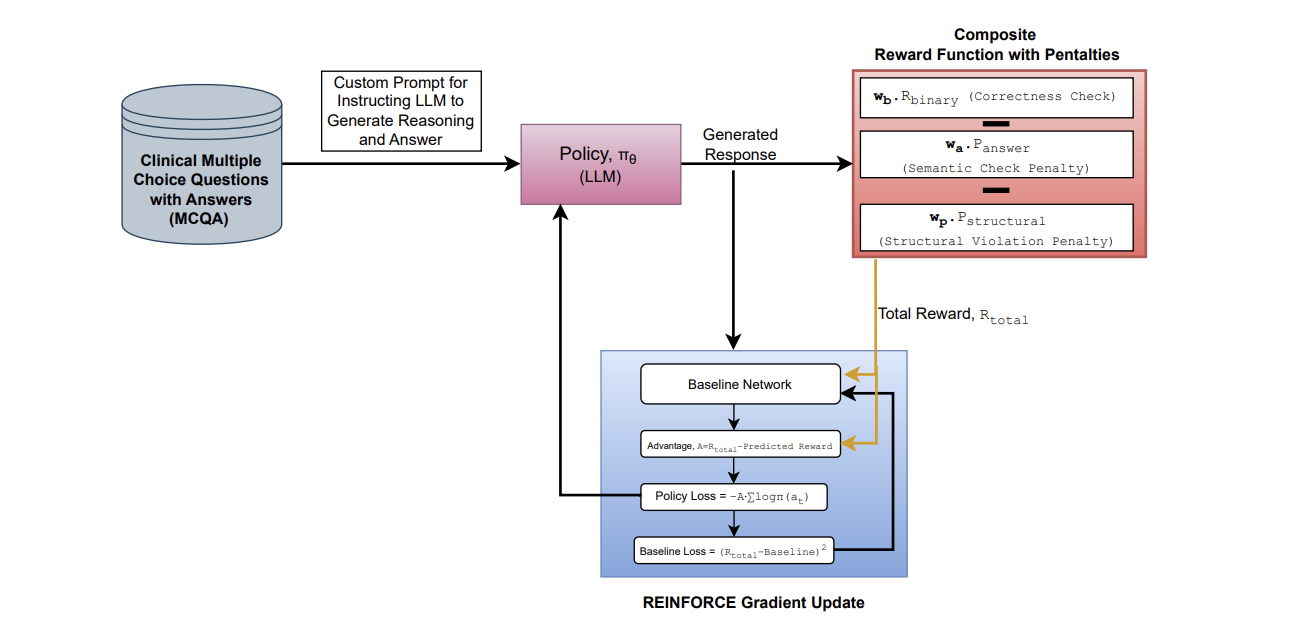
\includegraphics[width=\linewidth]{images/ Training_LLM with_Composite_RM.png}
    \caption{Обучение LLM по предложенной модели комплексного вознаграждения}
    \label{fig:Comp_RM}
\end{figure}

\subsection{Наборы данных}

В работе используются два набора данных для вопросов множественного выбора 
в медицинской области.

\begin{itemize}
    \item \emph{Набор MedQA-USMLE-4-options.}~\cite{jin2020medqa}  
    Набор содержит вопросы из экзаменов по медицине формата USMLE с четырьмя 
    вариантами ответов и подробными клиническими сценариями. Для обучения 
    используется $1000$ примеров, для тестирования~-- $200$ примеров из 
    той же выборки, пример см. на Рисунке~\ref{fig:MedQA-USMLE}. 

    \item \emph{Поднабор «Здоровье» из MMLU-PRO.}~\cite{wang2024mmlu}
    Этот набор покрывает широкий спектр задач по биологии и здравоохранению 
    и используется как внераспределительный тест (out-of-distribution). 
    Для тестирования берутся $200$ примеров. Описание и ссылка на набор 
    даны в работе по MMLU-PRO.
\end{itemize}

\begin{figure}
    \centering
    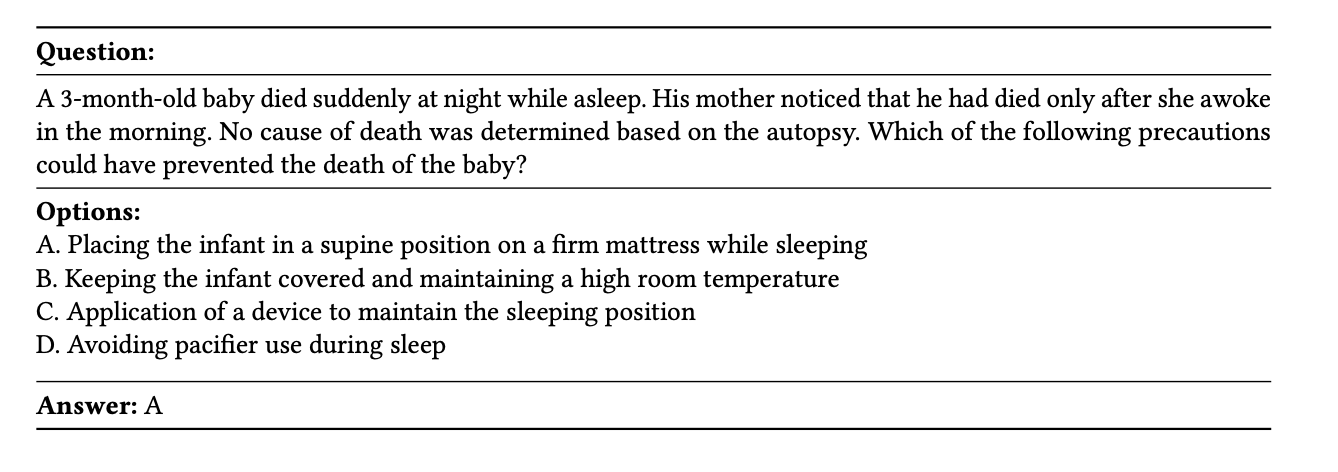
\includegraphics[width=\linewidth]{images/example_question_MedQA-USMLE_dataset.png}
    \caption{Пример вопроса из набора данных MedQA-USMLE}
    \label{fig:MedQA-USMLE}
\end{figure}

\subsection{Метрики}

Основные метрики, используемые в статье, можно разделить на несколько групп:

\paragraph{Точность ответа.}
    \begin{itemize}
        \item Доля вопросов, для которых финальный вариант $a_g$ совпадает 
        с правильным $a^*$.
        \item Отдельно оценивается для in-distribution (MedQA-USMLE) и 
        out-of-distribution (MMLU-PRO-Health).
    \end{itemize}

\paragraph{Частота взлома награды (hacking rate).}
    \begin{itemize}
        \item Доля сгенерированных ответов, в которых обнаружены:
        \begin{itemize}
            \item \emph{нарушения по ответу} (answer violation)~-- 
            семантическое утекание ответа в блоке \verb|<think>|,
            детектируемое по порогу $\tau_{\text{answer}}$;
            \item \emph{структурные нарушения} (structural violation)~--
            превышение длины прелюдии $|T_{\text{preamble}}| > \tau_{\text{preamble}}$.
        \end{itemize}
    \end{itemize}

\paragraph{Оценка по схеме «модель как судья».}
    \begin{itemize}
        \item Используются две внешние модели-судьи, которые оценивают 
        ответы по нескольким критериям:
        \begin{itemize}
            \item балл точности (шкала для оценки правильности),
            \item соблюдение формата (наличие и корректность тегов 
            \verb|<think>| и \verb|<answer>|),
            \item качество клинического рассуждения,
            \item безопасность ответа,
            \item степень взлома награды,
            \item степень утечки ответа.
        \end{itemize}
        \item Вычисляется коэффициент корреляции Пирсона между оценками 
        двух судей по каждому критерию.
    \end{itemize}

\paragraph{Человеческая предпочтительная оценка.}
    \begin{itemize}
        \item Группе испытуемых показывают пары ответов: один от базовой 
        модели, другой от модели с композитной наградой.
        \item Испытуемые выбирают: «лучше первый», «лучше второй», «оба», 
        «ни один».
        \item По результатам проводится критерий согласия (хи-квадрат) 
        для проверки отклонения распределения ответов от равномерного.
    \end{itemize}


\subsection{Модели}

В статье исследуются несколько конфигураций моделей.

\paragraph{Базовые инструкт-модели.}
    \begin{itemize}
        \item Модель семейства Llama версии с приблизительно трёхмиллиардным 
        числом параметров, ориентированная на инструктивные 
        задания~\cite{llama3techreport}.

        \item Модель семейства Qwen версии сопоставимого размера, 
        также предназначенная для инструктивных задач~\cite{qwen2.5}.
    \end{itemize}

\paragraph{Модели после дообучения с учителем (с рассуждением).}
    \begin{itemize}
        \item Каждая базовая модель дообучается в формате, где для 
        каждого вопроса задаётся требование:
        \begin{itemize}
            \item строить пошаговое клиническое рассуждение внутри \verb|<think>|,
            \item затем выводить букву ответа внутри \verb|<answer>|.
        \end{itemize}
        \item Дообучение проводится методом низкоранговой адаптации 
        параметров (LoRA) с квантованием до 4 бит по весам, чтобы уменьшить 
        требования к памяти.
    \end{itemize}

\paragraph{Модели с композитной наградой.}
    \begin{itemize}
        \item Поверх дообученных с учителем моделей применяется RL 
        с композитной функцией награды:
        \begin{itemize}
            \item бинарная награда за корректный ответ в правильном формате;
            \item штраф за семантическое утекание ответа в блоке \verb|<think>|;
            \item штраф за структурные нарушения (слишком длинный 
            пролог до \verb|<think>|).
        \end{itemize}
        \item Для оценки стабильности и улучшения формирования награды 
        используется сеть-базис, принимающая усреднённое скрытое 
        состояние финальных токенов.
    \end{itemize}

\paragraph{Модели-судьи.}
    \begin{itemize}
        \item Для экспертной автоматической оценки рассуждений и формата 
        используются две отдельные модели: универсальная масштабная модель 
        и специализированная медицинская модель MedGemma~\cite{medgemma2025}.
    \end{itemize}